%%%%%%%%%%%%%%%%%%%%%%%%%%%%%%%%%%%%%%%%%
% University Assignment Title Page 
% LaTeX Template
% Version 1.0 (27/12/12)
%
% This template has been downloaded from:
% http://www.LaTeXTemplates.com
%
% Original author:
% WikiBooks (http://en.wikibooks.org/wiki/LaTeX/Title_Creation)
%
% License:
% CC BY-NC-SA 3.0 (http://creativecommons.org/licenses/by-nc-sa/3.0/)
% 
% Instructions for using this template:
% This title page is capable of being compiled as is. This is not useful for 
% including it in another document. To do this, you have two options: 
%
% 1) Copy/paste everything between \begin{document} and \end{document} 
% starting at \begin{titlepage} and paste this into another LaTeX file where you 
% want your title page.
% OR
% 2) Remove everything outside the \begin{titlepage} and \end{titlepage} and 
% move this file to the same directory as the LaTeX file you wish to add it to. 
% Then add \input{./title_page_1.tex} to your LaTeX file where you want your
% title page.
%
%%%%%%%%%%%%%%%%%%%%%%%%%%%%%%%%%%%%%%%%%
%\title{Title page with logo}
%----------------------------------------------------------------------------------------
%	PACKAGES AND OTHER DOCUMENT CONFIGURATIONS
%----------------------------------------------------------------------------------------

\documentclass[12pt]{article}
\usepackage[english]{babel}
\usepackage[utf8x]{inputenc}
\usepackage{amsmath}
\usepackage{graphicx}
\usepackage[colorinlistoftodos]{todonotes}
\usepackage{listings}
\usepackage{color}
\usepackage{url}
\usepackage{booktabs}
\usepackage{hyperref}

\definecolor{codegreen}{rgb}{0,0.6,0}
\definecolor{codegray}{rgb}{0.5,0.5,0.5}
\definecolor{codepurple}{rgb}{0.58,0,0.82}
\definecolor{backcolour}{rgb}{0.95,0.95,0.92}
 
\lstdefinestyle{mystyle}{
    backgroundcolor=\color{backcolour},   
    commentstyle=\color{codegreen},
    keywordstyle=\color{magenta},
    numberstyle=\tiny\color{codegray},
    stringstyle=\color{codepurple},
    basicstyle=\footnotesize,
    breakatwhitespace=false,         
    breaklines=true,                 
    captionpos=b,                    
    keepspaces=true,                 
    numbers=left,                    
    numbersep=5pt,                  
    showspaces=false,                
    showstringspaces=false,
    showtabs=false,                  
    tabsize=2
}

\lstset{style=mystyle}

\textheight=250truemm \textwidth=160truemm 
\hoffset=-10truemm \voffset=-20truemm

\begin{document}

\begin{titlepage}

\newcommand{\HRule}{\rule{\linewidth}{0.5mm}} % Defines a new command for the horizontal lines, change thickness here

\center % Center everything on the page
 
%----------------------------------------------------------------------------------------
%	HEADING SECTIONS
%----------------------------------------------------------------------------------------

\textsc{\LARGE Ukrainian Catholic University}\\[1cm] % Name of your university/college
\textsc{\Large  Faculty of Applied Sciences}\\[0.5cm] % Major heading such as course name
\textsc{\large Data Science Master Programme}\\[0.5cm] % Minor heading such as course title

%----------------------------------------------------------------------------------------
%	TITLE SECTION
%----------------------------------------------------------------------------------------
\vspace*{1cm}

\HRule \\[0.4cm]
{ \huge \bfseries Images denoising using LPG-PCA algorithm}\\[10pt]
{\Large \bfseries Linear Algebra final project report}\\[0.4cm] % Title of your document
\HRule \\[1cm]
 
%----------------------------------------------------------------------------------------
%	AUTHOR SECTION
%----------------------------------------------------------------------------------------
\vspace*{1cm}

% If you don't want a supervisor, uncomment the two lines below and remove the section above
\Large \emph{Authors:}\\
Roman \textsc{Moiseiev}\\Teodor \textsc{Romanus}\\[1cm] % Your name

%----------------------------------------------------------------------------------------
%	DATE SECTION
%----------------------------------------------------------------------------------------
\vspace*{1cm}
{\large 24 January 2019}\\[2cm] % Date, change the \today to a set date if you want to be precise

%----------------------------------------------------------------------------------------
%	LOGO SECTION
%----------------------------------------------------------------------------------------


\includegraphics[height=5cm]{UCU-Apps.png}\\[1cm] % Include a department/university logo - this will require the graphicx package
 
%----------------------------------------------------------------------------------------

\vfill % Fill the rest of the page with whitespace

\end{titlepage}

\begin{abstract}
In this paper, we explore one of the images denoising algorithms, called LPG-PCA (Local Pixel Grouping – Principal Component Analysis). We provide a self-written implementation in Python and do comparisons with another filtering images denoising algorithms. 

Images taken with a camera can have noise from a variety of sources. Further use of these images requires the noise being reduced – for aesthetic purposes as in artistic work or marketing, or for practical purposes such as computer vision. 

The motivation for selecting the PCA-based algorithm is because one of the researchers finds PCA an interesting area to do some practice in. Another researcher works in the field of Computer Vision, and image processing tools are of very interest of him.
\end{abstract}

\section{Problem Setting}
Image noise is known irritation. Images taken with both digital cameras and conventional film cameras will pick up noise from a variety of sources, such as the film grain of analog cameras, sensor noise of digital cameras or analog-to-digital image transformations.  

We need to remove noise in images in several cases – for aesthetic purposes, such as artistic work or in marketing, or practical purposes such as computer vision.  

Noise can be random or white noise with an even frequency distribution, or frequency dependent noise introduced by a device's mechanism or signal processing algorithms. So, image noise can have very structure and (maybe) need a distinct algorithm for each noise origin. The most promising algorithms are those which efficiently deal with all image noises.

\section{Related Work}
The algorithm was first introduced in 2010 in \cite{zhang2010two}.  

At the same years (2005-2010), noise removal has been extensively studied and many denoising schemes have been proposed, from the earlier smoothing filters and frequency domain denoising method to the lately developed wavelet, curvelet and ridgelet based methods, sparse representation and K-SVD methods, shape-adaptive transform, bilateral filtering, non-local mean-based methods and non-local collaborative filtering \cite{zhang2010two}. One of the recent trends is Deep Learning, which in the form of deep CNN is applied to this problem. \cite{zhang2017beyond}. 

\section{Approach to Solution}
In this project, we implement the efficient image denoising algorithm which uses principal component analysis (PCA) with local pixel grouping (LPG) \cite{zhang2010two}. 

\textbf{The advantages of this algorithm are:}
\begin{itemize}
    \item Local pixel grouping allows preserving local features such as edges better. Pixel and its neighbours are modelled as vector variable. And samples for that variable are taken from the local window by using block matching LPG. 
    \item The algorithm may be applied more than one time (original paper uses two) which improve results. 
\end{itemize}

\textbf{The disadvantages are:}
\begin{itemize}
    \item Slow computations 1-2 minutes for the 256x256 image. For color images the training samples selected in local window L x L x 3 which increase computational costs.
    \item Also, color vector due to higher dimensionality requires more training samples which may reduce quality. 
    \item Applying the algorithm more than one time is required only for strong noise. 
    \item This algorithm isn’t the best choice for preserving large-grain edges and denoising smoothing areas. 
\end{itemize}

\subsection{Background}
After a lot of researching, we found that almost all papers regarding the theme of the research are mainly comparison-oriented: they used the implementation from the \cite{zhang2010two} and ran the algorithm against another image denoising algorithms. So, we had a poor choice.

The authors’ algorithm was not very good written and documented, and it was tough to map it with the formulas from the paper. It is written in MATLAB. 

Another iteration of research got us the very good implemented and documented solution\cite{image_denoising} in the Julia programming language, which, however, was only the part of the full solution of noise reducing task. Moreover, the author claimed that one picture took 26 minutes to process, and it wasn’t acceptable.

\subsection{Transition}
Because of all the researchers know Python, we decided to implement the LPG-PCA algorithm in Python. The algorithm should be at least the same for all these categories:
\begin{itemize}
    \item Denoising accuracy;
    \item Speed of work;
    \item Source code quality.
\end{itemize}
As a matter of fact, we preserved 1\textsuperscript{th} and 3\textsuperscript{rd} properties, and made the algorithm a lot faster with the parallel implementation.

\subsection{Foreground}
The main goal of the project is to get in touch with something new in Linear Algebra field, select one algorithm, implement it and compare it with another. 

Because of all that, we will be evaluating our LPG-PCA implementation with another image denoising filters: median filter, block-matching and 3D filtering (BM3D)\cite{dabov2006image}, non-local means filter (NLM) \cite{buades2005non}. We selected these filters because they showed good denoising results in other papers. 

The evaluation of results will be used with the next quality estimation techniques: 
\begin{itemize}
    \item Peak signal-to-noise ratio (PSNR) 
    \item Structural similarity index (SSIM) 
\end{itemize}
These image quality metrics are widely used in the papers, which defined out choice. 

The success of the solution (the algorithm implementation) defines by what PSNR and SSIM values we get from the original MATLAB implementation and our Python implementation. 

\section{Solution}

We choose LPG-PCA algorithm in order to resolve the task of denoising of the \emph{white additive noise} with preservation of edges structure. This algorithm based on the assumption that valuable signal in the image is concentrated on a small local part of image, but the noise is evenly distributed across the entire image. 

In order to exploit this idea, the Local pixel grouping is used. With this technique, we model pixel, which should be denoised, and the block of surrounding pixels as a vector variable. Training samples for this variable are similar blocks from the neighbourhood of the target block. After that, training matrix with most similar blocks, represented as vectors, moved to the PCA domain. Where signal and noise can be better distinguished. This is achieved by following a set of operations in the pseudocode below. Besides, that described above operations runs twice, in order to improve SSIM and visual quality of the denoised image.
Please NOTE that this code below matches our numerical implementation in Python \cite{our_github}, and variable names match original paper notation \cite{zhang2010two}.

\subsection{Pseudocode}
\begin{lstlisting}[escapeinside={(*}{*)}]
(*$K$*) = K; (*$L$*)=L; (*$\sigma$*)=sig
for pixel in pixels:
    # Get Block with length K for the target pixel
    target = getBlock(pixel.x, pixel.y)
    
    # Length of the block vector
    m = (*$K^2$*)
    
    # The desired number of the vector variables for the training matrix
    n = m * 8 + 1 

    # Get all possible blocks in (*$L$*) window around the pixel. There are (*$(L-K+1)^2$*) such blocks
    blocks = []
    for x in windowX: 
        for y in windowY:
            blocks.append(getBlock(x, y))
    
    # Sort blocks by similarity (MSE) with the target in Descending order
    blocks.sort(key = 'mse', order = 'desc')

    # If there are less than n - desired number of vector variables we will use all of them
    if blocks.length < n:
        n = blocks.length
    
    # Form training matrix as target and n most similar blocks
    (*$X_\nu$*) = concatenate(target, blocks[:n])

    # Remove mean from the training matrix on the length of block axis
    (*$\mu$*) = mean((*$X_\nu$*), axis = 1)
    (*$X_\nu = X_\nu - \mu$*)

    # Noise covariance is (*$\sigma^2 \times I$*)
    (*$\Omega_\nu = \sigma^2I$*)

    # Get eigenvectors of the input covariance matrix
    (*$\Omega_{\bar{X}_\nu}$*) = (*$\dfrac{1}{n}\bar{X}_\nu\bar{X}_\nu^\top$*)
    (*$\Phi_{\bar{X}}$*) = getEigenvectors((*$\Omega_{\bar{X}_\nu}$*))
    (*$P_{\bar{X}} = \Phi_{\bar{X}}^\top$*)
    
    # Get decorrelated dataset
    (*$\bar{Y}_\nu = P_{\bar{X}} X_\nu$*)

    # Get the covariance matrix of the transformed noise
    (*$\Omega_{\nu_y} = P_{\bar{X}} \Omega_\nu P_{\bar{X}}^\top$*)

    # Get the covariance matrix of the transformed input
    (*$\Omega_{\bar{y}_\nu} = \dfrac{1}{n}\bar{Y}_\nu \bar{Y}_\nu^\top$*)
    
    # Get the covariance matrix of the transformed denoised output
    (*$\Omega_{\bar{y}} = \Omega_{\bar{y}_\nu} - \Omega_{\nu_y}$*)
    
    # Get shrinkage coefficients
    (*$w = \dfrac{diag(\Omega_{\bar{y}})}{diag(\Omega_{\bar{y}}) + diag(\Omega_{y_\nu})}$*)
    
    # Get the transformed denoised output of the target
    (*$\hat{\bar{Y}} = w \cdot \bar{Y}_\nu$*)
    (*$\hat{X} = P_{\hat{X}}^\top \cdot \hat{\bar{Y}} + \mu$*)
    
    (*$\hat{x_0} = \hat{X}$*)[m//2]
    return (*$\hat{x_0}$*)
\end{lstlisting}

\section{Evaluation}
In the proposed LPG-PCA denoising algorithm, most of the computational cost spend on LPG grouping and PCA transformation, and thus the complexity mainly depends on two parameters: the size K of the variable block and the size L of the training block. In LPG grouping, it requires $(2K^2−1) \cdot (L−K+1)^2$ additions, $K^2 \cdot (L−K+1)^2$ multiplications and $(L−K+1)^2$ "less than" logic operations. \cite{zhang2010two} 

\begin{center}

\end{center}
\begin{center}
\begin{tabular}{c c c c}
    & noised & 1 stage & 2 stage\\
    \rotatebox{90}{\qquad\qquad\quad$\sigma$=10} & 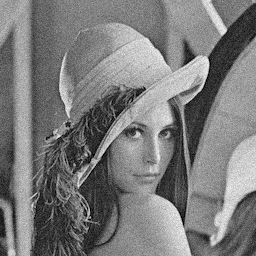
\includegraphics[width=50mm]{lena_noised_10.png} & 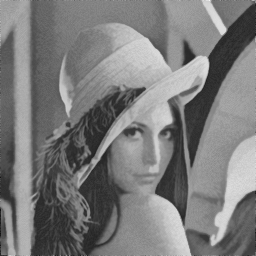
\includegraphics[width=50mm]{lena_interim_10.png} &
    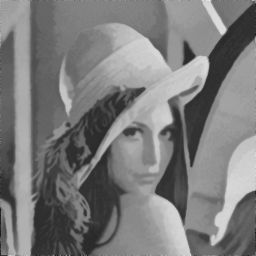
\includegraphics[width=50mm]{lena_denoised_10.png}\\
    \rotatebox{90}{\qquad\qquad\quad$\sigma$=20} & 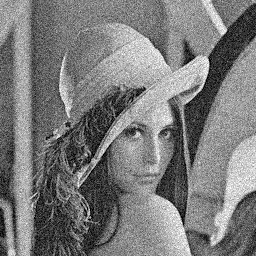
\includegraphics[width=50mm]{lena_noised_20.png} & 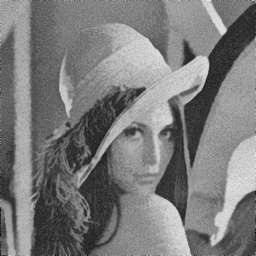
\includegraphics[width=50mm]{lena_interim_20.png} & 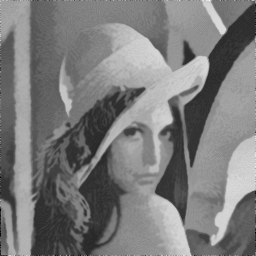
\includegraphics[width=50mm]{lena_denoised_20.png}\\
    \rotatebox{90}{\qquad\qquad\quad$\sigma$=30} & 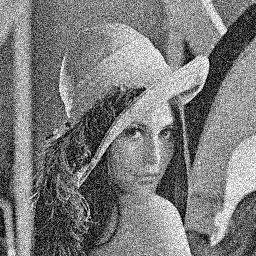
\includegraphics[width=50mm]{lena_noised_30.png} & 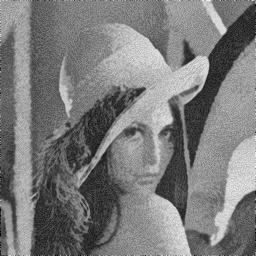
\includegraphics[width=50mm]{lena_interim_30.png} & 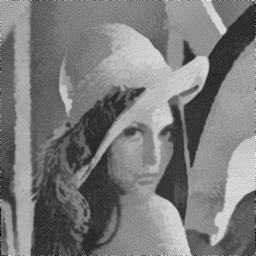
\includegraphics[width=50mm]{lena_denoised_30.png}\\
    \rotatebox{90}{\qquad\qquad\quad$\sigma$=40} & 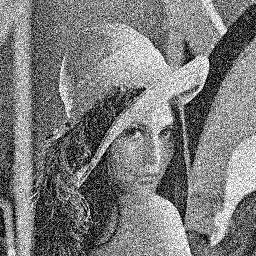
\includegraphics[width=50mm]{lena_noised_40.png} & 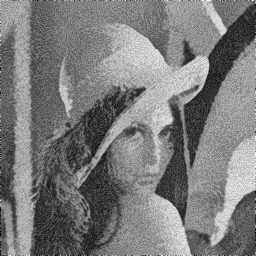
\includegraphics[width=50mm]{lena_interim_40.png} & 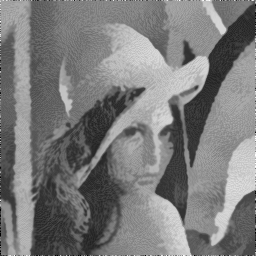
\includegraphics[width=50mm]{lena_denoised_40.png}\\
\end{tabular}

Figure 1. Noised image, denoised images on the 1\textsuperscript{st} and 2\textsuperscript{nd} steps of LPG-PCA.

\end{center}

\begin{center}
\begin{tabular}{c c c c}
    & house & hill & couple\\
    \rotatebox{90}{\qquad\qquad\quad LPG-PCA} & 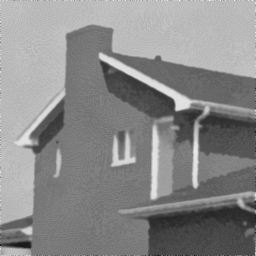
\includegraphics[width=50mm]{house_lpg_pca_20.png} & 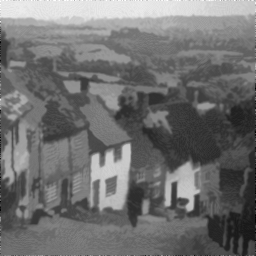
\includegraphics[width=50mm]{hill_lpg_pca_20.png} &
    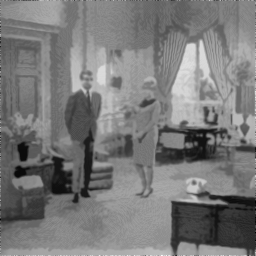
\includegraphics[width=50mm]{couple_lpg_pca_20.png}\\
    \rotatebox{90}{\qquad\qquad\quad MF} & 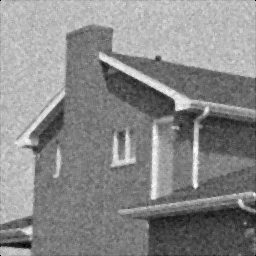
\includegraphics[width=50mm]{house_mf_20.png} & 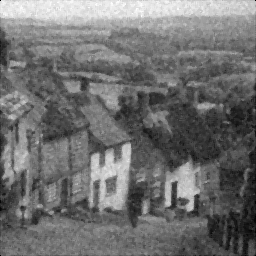
\includegraphics[width=50mm]{hill_mf_20.png} & 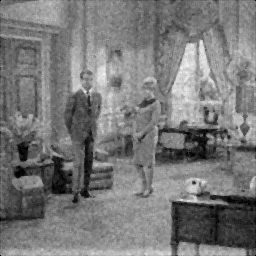
\includegraphics[width=50mm]{couple_mf_20.png}\\
    \rotatebox{90}{\qquad\qquad\quad NLM} & 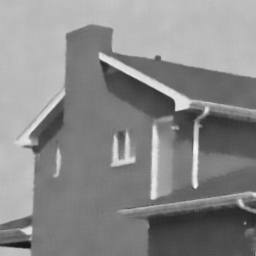
\includegraphics[width=50mm]{house_nlm_20.png} & 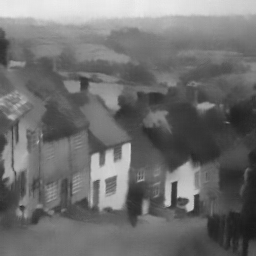
\includegraphics[width=50mm]{hill_nlm_20.png} & 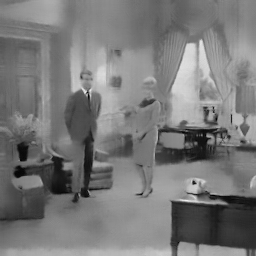
\includegraphics[width=50mm]{couple_nlm_20.png}\\
    \rotatebox{90}{\qquad\qquad\quad BM3D} & 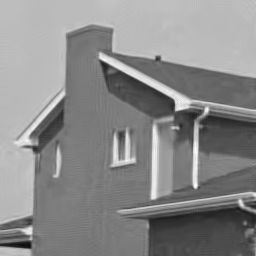
\includegraphics[width=50mm]{house_bm3d_20.png} & 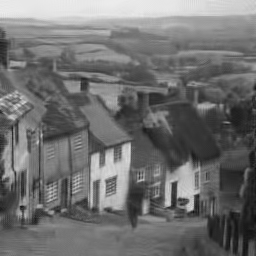
\includegraphics[width=50mm]{hill_bm3d_20.png} & 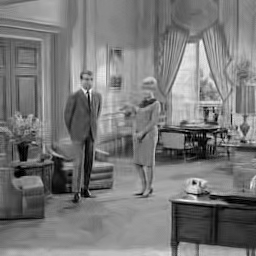
\includegraphics[width=50mm]{couple_bm3d_20.png}\\
\end{tabular}

Figure 2. Comparison of the different algorithms with $\sigma$=20.

\end{center}

For the computations, we used Python 3.6. It also worth to mention that Python implementation of the BM3D works only on the Mac and Linux.\cite{pybm3d}

We compared four algorithms: LPG-PCA, median filter, NLM and BM3D on the set of 12 monochrome pictures with different $\sigma$ = [10, 20, 30, 40]. Data in the table has the format PSNR(SSIM):

{\tiny
\noindent\begin{minipage}{.5\linewidth}
\begin{tabular}{lrrrr}
\toprule &&boat\\ \midrule
$\sigma$&LPG-PCA&MF&NLM&BM3D\\
\midrule
10&26.75(0.88)&26.73(0.88)&26.69(0.84)&33.77(0.96)\\
20&25.65(0.84)&25.11(0.8)&26.43(0.84)&30.07(0.93)\\
30&24.63(0.8)&23.44(0.71)&25.78(0.82)&28.27(0.9)\\
40&23.68(0.75)&21.88(0.62)&24.74(0.78)&26.61(0.87)\\
\bottomrule
\end{tabular}
\end{minipage}
\noindent\begin{minipage}{.5\linewidth}
\begin{tabular}{lrrrr}
\toprule &&hill\\ \midrule
$\sigma$&LPG-PCA&MF&NLM&BM3D\\
\midrule
10&28.69(0.89)&28.89(0.89)&26.88(0.81)&36.52(0.97)\\
20&27.31(0.85)&26.61(0.81)&26.7(0.81)&33.47(0.95)\\
30&26.0(0.81)&24.46(0.72)&26.16(0.79)&31.72(0.93)\\
40&24.75(0.75)&22.61(0.63)&25.23(0.76)&30.08(0.91)\\
\bottomrule
\end{tabular}
\end{minipage}
\noindent\begin{minipage}{.5\linewidth}
\begin{tabular}{lrrrr}
\toprule &&lena\\ \midrule
$\sigma$&LPG-PCA&MF&NLM&BM3D\\
\midrule
10&29.19(0.93)&29.45(0.92)&28.8(0.9)&32.35(0.95)\\
20&27.7(0.9)&26.82(0.83)&28.43(0.9)&28.69(0.89)\\
30&26.36(0.85)&24.54(0.73)&27.57(0.88)&26.9(0.85)\\
40&25.12(0.81)&22.64(0.64)&26.26(0.84)&25.5(0.81)\\
\bottomrule
\end{tabular}
\end{minipage}
\noindent\begin{minipage}{.5\linewidth}
\begin{tabular}{lrrrr}
\toprule &&house\\ \midrule
$\sigma$&LPG-PCA&MF&NLM&BM3D\\
\midrule
10&31.72(0.94)&31.46(0.91)&31.39(0.93)&30.18(0.98)\\
20&29.9(0.91)&27.94(0.81)&30.85(0.92)&26.2(0.94)\\
30&28.16(0.86)&25.22(0.7)&29.71(0.91)&24.24(0.9)\\
40&26.58(0.81)&23.08(0.59)&28.06(0.86)&22.99(0.86)\\
\bottomrule
\end{tabular}
\end{minipage}
\noindent\begin{minipage}{.5\linewidth}
\begin{tabular}{lrrrr}
\toprule &&mri\\ \midrule
$\sigma$&LPG-PCA&MF&NLM&BM3D\\
\midrule
10&28.13(0.86)&22.42(0.87)&26.99(0.85)&32.73(0.96)\\
20&22.11(0.66)&21.76(0.79)&26.5(0.84)&28.88(0.91)\\
30&18.59(0.5)&20.86(0.71)&25.5(0.82)&26.82(0.87)\\
40&16.09(0.4)&19.88(0.62)&24.12(0.78)&25.05(0.81)\\
\bottomrule
\end{tabular}
\end{minipage}
\noindent\begin{minipage}{.5\linewidth}
\begin{tabular}{lrrrr}
\toprule &&couple\\ \midrule
$\sigma$&LPG-PCA&MF&NLM&BM3D\\
\midrule
10&26.84(0.87)&26.76(0.87)&26.02(0.81)&36.55(0.98)\\
20&25.61(0.83)&25.16(0.79)&25.82(0.81)&32.62(0.96)\\
30&24.59(0.79)&23.47(0.71)&25.29(0.79)&30.32(0.94)\\
40&23.63(0.74)&21.92(0.62)&24.4(0.76)&27.75(0.91)\\
\bottomrule
\end{tabular}
\end{minipage}
\noindent\begin{minipage}{.5\linewidth}
\begin{tabular}{lrrrr}
\toprule &&peppers\\ \midrule
$\sigma$&LPG-PCA&MF&NLM&BM3D\\
\midrule
10&29.0(0.94)&30.15(0.93)&29.15(0.92)&34.31(0.97)\\
20&27.56(0.9)&27.24(0.85)&28.63(0.91)&30.88(0.94)\\
30&26.2(0.86)&24.78(0.75)&27.62(0.9)&28.94(0.92)\\
40&24.97(0.82)&22.78(0.65)&26.18(0.86)&27.13(0.88)\\
\bottomrule
\end{tabular}
\end{minipage}
\noindent\begin{minipage}{.5\linewidth}
\begin{tabular}{lrrrr}
\toprule &&montage\\ \midrule
$\sigma$&LPG-PCA&MF&NLM&BM3D\\
\midrule
10&27.32(0.95)&27.77(0.93)&31.69(0.95)&32.91(0.96)\\
20&26.39(0.91)&26.04(0.83)&30.82(0.95)&29.06(0.91)\\
30&25.35(0.87)&24.14(0.72)&29.37(0.93)&27.03(0.87)\\
40&24.28(0.81)&22.39(0.61)&27.54(0.88)&25.56(0.83)\\
\bottomrule
\end{tabular}
\end{minipage}
\noindent\begin{minipage}{.5\linewidth}
\begin{tabular}{lrrrr}
\toprule &&fingerprint\\ \midrule
$\sigma$&LPG-PCA&MF&NLM&BM3D\\
\midrule
10&24.52(0.9)&23.46(0.88)&23.85(0.85)&34.03(0.97)\\
20&23.35(0.86)&22.25(0.84)&23.49(0.84)&30.42(0.94)\\
30&22.28(0.83)&21.08(0.8)&22.71(0.83)&28.45(0.9)\\
40&21.31(0.79)&19.99(0.76)&21.59(0.79)&26.9(0.87)\\
\bottomrule
\end{tabular}
\end{minipage}
\noindent\begin{minipage}{.5\linewidth}
\begin{tabular}{lrrrr}
\toprule &&cameraman\\ \midrule
$\sigma$&LPG-PCA&MF&NLM&BM3D\\
\midrule
10&27.26(0.91)&26.56(0.88)&29.13(0.9)&34.74(0.97)\\
20&26.2(0.87)&25.03(0.79)&28.58(0.9)&30.93(0.94)\\
30&25.17(0.83)&23.35(0.68)&27.52(0.88)&28.87(0.91)\\
40&24.16(0.77)&21.8(0.58)&26.07(0.84)&27.21(0.88)\\
\bottomrule
\end{tabular}
\end{minipage}
\noindent\begin{minipage}{.5\linewidth}
\begin{tabular}{lrrrr}
\toprule &&man\\ \midrule
$\sigma$&LPG-PCA&MF&NLM&BM3D\\
\midrule
10&27.51(0.88)&28.08(0.89)&26.78(0.83)&32.9(0.95)\\
20&26.31(0.85)&25.98(0.81)&26.55(0.83)&29.55(0.9)\\
30&25.2(0.81)&23.99(0.72)&25.94(0.81)&27.79(0.86)\\
40&24.15(0.76)&22.27(0.63)&24.97(0.78)&26.49(0.82)\\
\bottomrule
\end{tabular}
\end{minipage}
\noindent\begin{minipage}{.5\linewidth}
\begin{tabular}{lrrrr}
\toprule &&barbara\\ \midrule
$\sigma$&LPG-PCA&MF&NLM&BM3D\\
\midrule
10&28.38(0.92)&27.54(0.88)&27.96(0.88)&32.77(0.96)\\
20&26.93(0.88)&25.74(0.81)&27.59(0.88)&28.97(0.91)\\
30&25.68(0.85)&23.9(0.73)&26.75(0.86)&27.03(0.87)\\
40&24.52(0.8)&22.25(0.65)&25.51(0.82)&25.56(0.83)\\
\bottomrule
\end{tabular}
\end{minipage}
}

All images used can be found in the GitHub repository [6].

The data from table show that the LPG-PCA algorithm works well in comparison with median filter and non-local means on low noise data, but work less effective with larger noise data. In the case of the BM3D, this state of the art algorithm by our experiments is superior to all algorithms that we used in the evaluation.

\section{Conclusions}
In this project, we have explored the Local Pixel Grouping – Principal Component Analysis (LPG-PCA) algorithm. We have implemented the algorithm in Python and run its comparison with another popular algorithm. 

In the result that LPG-PCA has it's pros, in the form of preserving edges, and cons in the form of slow computation. PSNR and SSIM in original paper were calculated with truncating 20 border pixels, which introduced some restrictions, that do not exist for non-local algorithms. In comparison, the results from the BM3D looks more convenient for images that we used.

The obtained result has a somewhat smaller PSNR and SSIM measurements in comparison to original work but runs a lot faster. We think it may be because truncation of 20 border pixels is $\approx 28\%$ of the image. And measurements for the original paper were on truncated images, however, we performed them on the whole image. Also, original paper have complex tuned hyperparameters, which also affect quality.

What can be improved:

\begin{itemize}
    \item Since we work only with monochrome images and LPG-PCA algorithm for color images in Python could be implemented in future. 
    \item Also, there are a lot of hyperparameters which could be tuned. As the algorithm is very parallelable, due to the fact that each pixel could be denoised separately, the next logical step is to implement it on GPUs. 
    \item With that, it can run hundreds of times faster, and this will open a whole new world of hyperparameters tuning and possible accuracy improving.
\end{itemize}

What cannot be improved:

\begin{itemize}
    \item Due to the nature of the algorithm it will not be the best option for the denoising of the images with large-grain edges, and smooth areas.
\end{itemize}

Looking at all results, we could say, that LPG-PCA is not the fastest or most accurate algorithm, so its’ use in 2019 is unjustified. However, an idea behind the original paper is interesting and may be reused in the future.

\bibliographystyle{unsrt}%Used BibTeX style is unsrt
\bibliography{references}

\end{document}